\chapter{Theoretische Grundlagen und Definitionen}

Das folgende Kapitel dient der Bereitstellung von Grundlagenwissen zu in der Arbeit verwendeten Konzepten bereit. Detaillierte Ausführungen finden sich in den im Literaturverzeichnis aufgeführten Werken wieder. Zusätzlich werden Definitionen festgelgt.
Dient der theroethischen Fundiuerng. Dabeiw erden grundlegende Konzepte zu den Themen Kreativität, experimentelle Forschung, Wirtschaftsinformatik und der Geschäftsmodelltheorie gegeben.


\newpage

\newcommand{\abstand}{.35cm}
\begin{table}[H]
\centering
\caption{Überblick experimenteller Designs}
\label{my-label}
\resizebox{\textwidth}{!}{%
\begin{tabular}{L{0.03\textwidth}L{0.35\textwidth}C{0.15\textwidth}C{0.25\textwidth}@{}R{0.05\textwidth}@{}C{0.45\textwidth}@{}}
\toprule
               \textbf{ID} &                                  \textbf{Design}        &                      \textbf{Analyseeinheit} & \textbf{Kontrolltechnik} && \textbf{Versuchsanordnung/Bedingungsvariation} \\ \midrule
\textbf{1}             &\textbf{Zufallsgruppenpläne}&&&&\\
1.1 &  Solomon Four-Group   & G1   & R &&  \begin{tabular}[c]{C{\abstand}C{\abstand}C{\abstand}C{\abstand}C{\abstand}C{\abstand}C{\abstand}}&$\mathcal{O}_{~}$&&\multicolumn{2}{C{1.1cm}}{$\chi$}&&$\mathcal{O}_{+}$\end{tabular}              \\
 &  & G2 & R &&  \begin{tabular}[c]{C{\abstand}C{\abstand}C{\abstand}C{\abstand}C{\abstand}C{\abstand}C{\abstand}}&$\mathcal{O}_{~}$&&\multicolumn{2}{C{1.1cm}}{--}&&$\mathcal{O}_{+}$\end{tabular}        \\ 
  & & G3 & R && \begin{tabular}[c]{C{\abstand}C{\abstand}C{\abstand}C{\abstand}C{\abstand}C{\abstand}C{\abstand}}&--&&\multicolumn{2}{C{1.1cm}}{$\chi$}&&$\mathcal{O}_{+}$\end{tabular}          \\ 
  & & G4 & R && \begin{tabular}[c]{C{\abstand}C{\abstand}C{\abstand}C{\abstand}C{\abstand}C{\abstand}C{\abstand}}&--&&\multicolumn{2}{C{1.1cm}}{--}&&$\mathcal{O}_{+}$\end{tabular}   \\
  & &&&&\\
1.2  & Pretest-Postest Control Group                          & G1  &  R && \begin{tabular}[c]{C{\abstand}C{\abstand}C{\abstand}C{\abstand}C{\abstand}C{\abstand}C{\abstand}}&$\mathcal{O}_{~}$&&\multicolumn{2}{C{1.1cm}}{$\chi$}&&$\mathcal{O}_{+}$\end{tabular}      \\ 
  & & G2 & R && \begin{tabular}[c]{C{\abstand}C{\abstand}C{\abstand}C{\abstand}C{\abstand}C{\abstand}C{\abstand}}&$\mathcal{O}_{~}$&&\multicolumn{2}{C{1.1cm}}{--}&&$\mathcal{O}_{+}$\end{tabular} \\
  & &&&& \\                    
1.3  & Pretest-Only Control Group & G1 &  R && \begin{tabular}[c]{C{\abstand}C{\abstand}C{\abstand}C{\abstand}C{\abstand}C{\abstand}C{\abstand}}&--&&\multicolumn{2}{C{1.1cm}}{$\chi$}&&$\mathcal{O}_{+}$\end{tabular}        \\   
  &  &G2 & R && \begin{tabular}[c]{C{\abstand}C{\abstand}C{\abstand}C{\abstand}C{\abstand}C{\abstand}C{\abstand}}&--&&\multicolumn{2}{C{1.1cm}}{--}&&$\mathcal{O}_{+}$\end{tabular} \\ 
  &&&&&\\
 \textbf{2} &\textbf{Wiederholungsmessung}&&&&\\
 2.1& Balanciert  &  &   && \begin{tabular}[c]{C{\abstand}C{\abstand}C{\abstand}C{\abstand}C{\abstand}C{\abstand}C{\abstand}}& \multicolumn{6}{c}{\;\; Stimulus-Position} \end{tabular}    \\ 
 &   &  &    && \begin{tabular}[c]{C{\abstand}C{\abstand}C{\abstand}C{\abstand}C{\abstand}C{\abstand}C{\abstand}}& I &II&III&IV&V&VI  \end{tabular}    \\
 &   & P1 &  W(R)  && \begin{tabular}[c]{C{\abstand}C{\abstand}C{\abstand}C{\abstand}C{\abstand}C{\abstand}C{\abstand}}&$\chi_{1}$&$\mathcal{O}_{+}$&$\chi_{2}$&$\mathcal{O}_{+}$&$\chi_{3}$&$\mathcal{O}_{+}$\end{tabular}    \\   
& &P2 &W(R)&& \begin{tabular}[c]{C{\abstand}C{\abstand}C{\abstand}C{\abstand}C{\abstand}C{\abstand}C{\abstand}}&$\chi_{1}$&$\mathcal{O}_{+}$&$\chi_{3}$&$\mathcal{O}_{+}$&$\chi_{2}$&$\mathcal{O}_{+}$\end{tabular} \\
& &P3 &W(R)&& \begin{tabular}[c]{C{\abstand}C{\abstand}C{\abstand}C{\abstand}C{\abstand}C{\abstand}C{\abstand}}&$\chi_{2}$&$\mathcal{O}_{+}$&$\chi_{1}$&$\mathcal{O}_{+}$&$\chi_{3}$&$\mathcal{O}_{+}$\end{tabular} \\
& &P4 &W(R)&& \begin{tabular}[c]{C{\abstand}C{\abstand}C{\abstand}C{\abstand}C{\abstand}C{\abstand}C{\abstand}}&$\chi_{2}$&$\mathcal{O}_{+}$&$\chi_{3}$&$\mathcal{O}_{+}$&$\chi_{1}$&$\mathcal{O}_{+}$\end{tabular} \\
&& P5 &W(R)&& \begin{tabular}[c]{C{\abstand}C{\abstand}C{\abstand}C{\abstand}C{\abstand}C{\abstand}C{\abstand}}&$\chi_{3}$&$\mathcal{O}_{+}$&$\chi_{1}$&$\mathcal{O}_{+}$&$\chi_{2}$&$\mathcal{O}_{+}$\end{tabular} \\
&& P6 &W(R)&& \begin{tabular}[c]{C{\abstand}C{\abstand}C{\abstand}C{\abstand}C{\abstand}C{\abstand}C{\abstand}}&$\chi_{3}$&$\mathcal{O}_{+}$&$\chi_{2}$&$\mathcal{O}_{+}$&$\chi_{1}$&$\mathcal{O}_{+}$\end{tabular} \\ 
&&&&&\\
 2.2& Nicht balanciert  &  &    && \begin{tabular}[c]{C{\abstand}C{\abstand}C{\abstand}C{\abstand}C{\abstand}C{\abstand}C{\abstand}}& \multicolumn{6}{c}{\;\; Stimulus-Position}\end{tabular}    \\ 
 &   &  &    && \begin{tabular}[c]{C{\abstand}C{\abstand}C{\abstand}C{\abstand}C{\abstand}C{\abstand}C{\abstand}}& I &II&III&IV&V&VI \end{tabular}    \\
  &   & P1 &  W(R)  && \begin{tabular}[c]{C{\abstand}C{\abstand}C{\abstand}C{\abstand}C{\abstand}C{\abstand}C{\abstand}}&$\chi_{1}$&$\mathcal{O}_{+}$&$\chi_{2}$&$\mathcal{O}_{+}$&$\chi_{3}$&$\mathcal{O}_{+}$\end{tabular}    \\ 
&  &P2 &W(R)&& \begin{tabular}[c]{C{\abstand}C{\abstand}C{\abstand}C{\abstand}C{\abstand}C{\abstand}C{\abstand}}&$\chi_{1}$&$\mathcal{O}_{+}$&$\chi_{2}$&$\mathcal{O}_{+}$&$\chi_{3}$&$\mathcal{O}_{+}$\end{tabular} \\
& &P3 &W(R)&& \begin{tabular}[c]{C{\abstand}C{\abstand}C{\abstand}C{\abstand}C{\abstand}C{\abstand}C{\abstand}}&$\chi_{1}$&$\mathcal{O}_{+}$&$\chi_{2}$&$\mathcal{O}_{+}$&$\chi_{3}$&$\mathcal{O}_{+}$\end{tabular} \\
& &P4 &W(R)&& \begin{tabular}[c]{C{\abstand}C{\abstand}C{\abstand}C{\abstand}C{\abstand}C{\abstand}C{\abstand}}&$\chi_{1}$&$\mathcal{O}_{+}$&$\chi_{2}$&$\mathcal{O}_{+}$&$\chi_{3}$&$\mathcal{O}_{+}$\end{tabular} \\
&& P5 &W(R)&& \begin{tabular}[c]{C{\abstand}C{\abstand}C{\abstand}C{\abstand}C{\abstand}C{\abstand}C{\abstand}}&$\chi_{1}$&$\mathcal{O}_{+}$&$\chi_{2}$&$\mathcal{O}_{+}$&$\chi_{3}$&$\mathcal{O}_{+}$\end{tabular} \\
&& P6 &W(R)&& \begin{tabular}[c]{C{\abstand}C{\abstand}C{\abstand}C{\abstand}C{\abstand}C{\abstand}C{\abstand}}&$\chi_{1}$&$\mathcal{O}_{+}$&$\chi_{2}$&$\mathcal{O}_{+}$&$\chi_{3}$&$\mathcal{O}_{+}$\end{tabular} \\ 
&&&&&\\
&&&&&\\
%5&Blockmessung/Parallelisierung&G1&B(R)&\multirow{5}{*}{\rotatebox[origin=c]{90}{Blockfaktor}}&\begin{tabular}[c]{C{\abstand}C{\abstand}C{\abstand}C{\abstand}C{\abstand}C{\abstand}}$\chi_{3}$&$\mathcal{O}$&$\chi_{2}$&$\mathcal{O}$&$\chi_{1}$&$\mathcal{O}$\end{tabular}\\
3&\textbf{Blockmessung/Parallelisierung}&G1&B(R)&\multirow{5}{*}{\rotatebox[origin=c]{90}{Blockfaktor} }&\begin{tabular}[c]{C{\abstand}C{\abstand}C{\abstand}C{\abstand}C{\abstand}C{\abstand}C{\abstand}}&$\chi_{1}$&$\chi_{2}$&$\chi_{3}$&$\chi_{4}$&$\chi_{5}$&$\chi_{6}$\end{tabular}\\
&& G2 &B(R)&& \begin{tabular}[c]{C{\abstand}C{\abstand}C{\abstand}C{\abstand}C{\abstand}C{\abstand}C{\abstand}}&$\chi_{1}$&$\chi_{2}$&$\chi_{3}$&$\chi_{4}$&$\chi_{5}$&$\chi_{6}$\end{tabular} \\ 
&& G3 &B(R)&& \begin{tabular}[c]{C{\abstand}C{\abstand}C{\abstand}C{\abstand}C{\abstand}C{\abstand}C{\abstand}}&$\chi_{1}$&$\chi_{2}$&$\chi_{3}$&$\chi_{4}$&$\chi_{5}$&$\chi_{6}$\end{tabular} \\ 
&& G4 &B(R)&& \begin{tabular}[c]{C{\abstand}C{\abstand}C{\abstand}C{\abstand}C{\abstand}C{\abstand}C{\abstand}}&$\chi_{1}$&$\chi_{2}$&$\chi_{3}$&$\chi_{4}$&$\chi_{5}$&$\chi_{6}$\end{tabular} \\ 
&& G5 &B(R)&& \begin{tabular}[c]{C{\abstand}C{\abstand}C{\abstand}C{\abstand}C{\abstand}C{\abstand}C{\abstand}}&$\chi_{1}$&$\chi_{2}$&$\chi_{3}$&$\chi_{4}$&$\chi_{5}$&$\chi_{6}$\end{tabular} \\  
&&&&&\\
&&&&&\\
4 & \textbf{Faktorielle (Misch-)Pläne}&&&&\\
4.1& Vollständig gekreuzter Plan  &  &    && \begin{tabular}[c]{C{\abstand}C{\abstand}C{\abstand}C{\abstand}C{\abstand}C{\abstand}C{\abstand}}&\multicolumn{6}{c}{Faktor B - R}  \end{tabular}    \\
&(5x6)&&&&\begin{tabular}[c]{C{\abstand}C{\abstand}C{\abstand}C{\abstand}C{\abstand}C{\abstand}C{\abstand}}& I &II&III&IV&V&VI  \end{tabular}\\
 &  &  & \multirow{5}{*}{\rotatebox[origin=c]{90}{R}}   &\multirow{5}{*}{\rotatebox[origin=c]{90}{Faktor A - R}}& \begin{tabular}[c]{R{\abstand}C{\abstand}C{\abstand}C{\abstand}C{\abstand}C{\abstand}C{\abstand}}I&$\chi_{11}$&$\chi_{12}$&$\chi_{13}$&$\chi_{14}$&$\chi_{15}$&$\chi_{16}$\end{tabular}    \\
 &  &  &    && \begin{tabular}[c]{R{\abstand}C{\abstand}C{\abstand}C{\abstand}C{\abstand}C{\abstand}C{\abstand}}II&$\chi_{21}$&$\chi_{22}$&$\chi_{23}$&$\chi_{24}$&$\chi_{25}$&$\chi_{26}$\end{tabular}    \\
  &  &  &    && \begin{tabular}[c]{R{\abstand}C{\abstand}C{\abstand}C{\abstand}C{\abstand}C{\abstand}C{\abstand}}III&$\chi_{31}$&$\chi_{32}$&$\chi_{33}$&$\chi_{34}$&$\chi_{35}$&$\chi_{36}$\end{tabular}    \\
   &  & &    && \begin{tabular}[c]{R{\abstand}C{\abstand}C{\abstand}C{\abstand}C{\abstand}C{\abstand}C{\abstand}}IV&$\chi_{41}$&$\chi_{42}$&$\chi_{43}$&$\chi_{44}$&$\chi_{45}$&$\chi_{46}$\end{tabular}    \\
    &  &  &    && \begin{tabular}[c]{R{\abstand}C{\abstand}C{\abstand}C{\abstand}C{\abstand}C{\abstand}C{\abstand}}V&$\chi_{51}$&$\chi_{52}$&$\chi_{53}$&$\chi_{54}$&$\chi_{55}$&$\chi_{56}$\end{tabular}    \\
 &&&&&\\   
4.1& Hierachischer Plan  &  &    && \begin{tabular}[c]{C{\abstand}C{\abstand}C{\abstand}C{\abstand}C{\abstand}C{\abstand}C{\abstand}}&\multicolumn{6}{c}{Faktor B - R}  \end{tabular}    \\
4.1& (5x6)  &  &    && \begin{tabular}[c]{C{\abstand}C{\abstand}C{\abstand}C{\abstand}C{\abstand}C{\abstand}C{\abstand}}& I &II&III&IV&V&VI \end{tabular}    \\
 &  &  & \multirow{5}{*}{\rotatebox[origin=c]{90}{R}}   &\multirow{5}{*}{\rotatebox[origin=c]{90}{Faktor A - R}}& \begin{tabular}[c]{R{\abstand}C{\abstand}C{\abstand}C{\abstand}C{\abstand}C{\abstand}C{\abstand}}I&$\chi_{11}$&$\chi_{12}$&$\chi_{13}$&$\chi_{14}$&$\chi_{15}$&$\chi_{16}$\end{tabular}    \\
 &  &  &    && \begin{tabular}[c]{R{\abstand}C{\abstand}C{\abstand}C{\abstand}C{\abstand}C{\abstand}C{\abstand}}II&&&&$\chi_{24}$&$\chi_{25}$&$\chi_{26}$\end{tabular}    \\
  &  &  &    && \begin{tabular}[c]{R{\abstand}C{\abstand}C{\abstand}C{\abstand}C{\abstand}C{\abstand}C{\abstand}}III&&&&$\chi_{34}$&$\chi_{35}$&$\chi_{36}$\end{tabular}    \\
   &  & &    && \begin{tabular}[c]{R{\abstand}C{\abstand}C{\abstand}C{\abstand}C{\abstand}C{\abstand}C{\abstand}}IV&$\chi_{41}$&$\chi_{42}$&$\chi_{43}$&&&\end{tabular}    \\
    &  &  &    && \begin{tabular}[c]{R{\abstand}C{\abstand}C{\abstand}C{\abstand}C{\abstand}C{\abstand}C{\abstand}}V&$\chi_{51}$&$\chi_{52}$&$\chi_{53}$&&&\end{tabular}    \\    
%&&  && \begin{tabular}[c]{C{\abstand}C{\abstand}C{\abstand}C{\abstand}C{\abstand}C{\abstand}}1&2&3&4&5&6\end{tabular} \\ 
\midrule 


 \multicolumn{6}{l}{\begin{footnotesize} G=Gruppe,\; P=Person,\; (R)/R=(eingeschränkte) Randomisierung, \; $\mathcal{O}_{~}$=Vormessung, \; $\mathcal{O}_{+}$=Nachmessung, \; $\chi$=Stimulus \end{footnotesize} }  \\ \bottomrule
                  
\section{Experiment}
\end{tabular}
}
\end{table}

\newpage

\newcommand{\test}{.40\textwidth}
\begin{table}[]
\centering
\caption{My caption}
\label{my-label}
\resizebox{\textwidth}{!}{%
\begin{tabular}{@{}C{0.05\textwidth}L{0.25\textwidth}@{}C{0.43\textwidth}@{}C{0.43\textwidth}@{}}
\toprule
 &  & \textbf{Stärken} & \textbf{Schwächen} \\   \midrule
               
\multirow{3}{*}{\rotatebox[origin=c]{90}{Design 1.1 -- 1.3 \;}} & Pretest-Only    &   \begin{tabular}[c]{@{}L{\test}@{}}   Dummytext Dummytext Dummytext Dummytext Dummytext Dummytext Dummytext Dummytext \end{tabular}     &      \begin{tabular}[c]{@{}L{\test}@{}}    Dummytext Dummytext Dummytext Dummytext Dummytext Dummytext Dummytext Dummytext \end{tabular}          \\
& Pretest-Postest     &   \begin{tabular}[c]{@{}L{\test}@{}}    Dummytext Dummytext Dummytext Dummytext Dummytext Dummytext Dummytext Dummytext \end{tabular}     &      \begin{tabular}[c]{@{}L{\test}@{}}    Dummytext Dummytext Dummytext Dummytext Dummytext Dummytext Dummytext Dummytext \end{tabular}      \\
& Solomon Four-Group   &   \begin{tabular}[c]{@{}L{\test}@{}}    Dummytext Dummytext Dummytext Dummytext Dummytext Dummytext Dummytext Dummytext \end{tabular}     &      \begin{tabular}[c]{@{}L{\test}@{}}    Dummytext Dummytext Dummytext Dummytext Dummytext Dummytext Dummytext Dummytext \end{tabular}    \\ \midrule
\multirow{3}{*}{\rotatebox[origin=c]{90}{Design 2.1 -- 2.3 \;}}&Randomisierung   &   \begin{tabular}[c]{@{}L{\test}@{}}    Dummytext Dummytext Dummytext Dummytext Dummytext Dummytext Dummytext Dummytext \end{tabular}     &      \begin{tabular}[c]{@{}L{\test}@{}}    Dummytext Dummytext Dummytext Dummytext Dummytext Dummytext Dummytext Dummytext \end{tabular}       \\
&Blockversuch     &       \begin{tabular}[c]{@{}L{\test}@{}}    Dummytext Dummytext Dummytext Dummytext Dummytext Dummytext Dummytext Dummytext \end{tabular}       &         \begin{tabular}[c]{@{}L{\test}@{}}    Dummytext Dummytext Dummytext Dummytext Dummytext Dummytext Dummytext Dummytext \end{tabular}   \\
&Messwiederholung &         \begin{tabular}[c]{@{}L{\test}@{}}    Dummytext Dummytext Dummytext Dummytext Dummytext Dummytext Dummytext Dummytext \end{tabular}     &      \begin{tabular}[c]{@{}L{\test}@{}}    Dummytext Dummytext Dummytext Dummytext Dummytext Dummytext Dummytext Dummytext \end{tabular}    \\ \bottomrule
\end{tabular}
}
\end{table}

\newpage

\begin{figure}[h]
\centering
\caption{Vergleich der Experimente, eigene Darstellung in Anlehnung an \cite{hewing}}
\resizebox{\textwidth}{!}{%

\begin{tikzpicture}
\tikzstyle{rechteck_bold}=[rechteck, font=\bfseries, draw=none, minimum height=1.5cm]
\node[rechteck] (5) at (-10.5,-3) {Bedingungskontrolle Sekundärvarianz möglich? (Ceteris paribus)};
\node [rechteck] (8) at (-2.5,-3) {Bedingungskontrolle Sekundärvarianz möglich? (Ceteris paribus)};
\node [rechteck](4) at (-6.5,0.5) {Werden Probandengruppen zufällig gebildet (nicht selegiert) und den Versuchsbedingungen oder -abfolgen zufällig zugewiesen?};
\node [rechteck](3) at (-3,3) {Werden mehrere Gruppen/Versuchsbedingungen untersucht?};
\node [rechteck] (2) at (0.5,5.5) {Bestimmt die unabhängige Variable die abhängige Variable? (uV -> aV)};
\node [rechteck](1) at (4,8) {Ist eine Unterscheidung von unabhängiger Variable (uV) und abhängiger Variable (aV) möglich?};
\node [rechteck] (11) at (9,2.5) {aV gegeben, uV gesucht};
\node [rechteck](10) at (9,5.5) {Korrelationsstudie \\(6)};
\node [rechteck](9) at (3,0.5) {Vorexperimentelle Versuchsanordnung (one-shot-case-study)\\(4)};
\node [rechteck] (13) at (5,-3) {Feldstudie \\(3)};
\node [rechteck_bold] (6) at (-14,-6) {(Labor)-Experiment\\(1.1)};
\node [rechteck_bold] (7) at (-8,-6) {Feld-Experiment\\(1.2)};
\node [rechteck_bold] (14) at (-2.5,-6) {Quasi-Experiment\\(2)};
\node [rechteck] (12) at (9,-0.5) {Ex-post-facto-Studie\\(5)};

\draw[pfeil_einfach] (1.west) -|  ++(0,0) -|  node[pos=.7, fill=white, rotate=0, align=center] {ja}(2.north);
\draw[pfeil_einfach] (2.west) -|  ++(0,0) -|  node[pos=.7,fill=white , rotate=0, align=center] {ja}(3.north);
\draw[pfeil_einfach] (3.west) -|  ++(0,0) -|  node[fill=white, pos=.7, rotate=0, align=center] {ja\\k<2}(4.north);
\draw[pfeil_einfach] (4.west) -|  ++(0,0) -|  node[fill=white, pos=.7, rotate=0, align=center] {ja}(5.north);
\draw[pfeil_einfach] (5.south) -|  ++(0,-.4) -|  node[fill=white, pos=.25, rotate=0, align=center] {nein}(7.north);
\draw[pfeil_einfach] (5.west) -|  ++(0,0) -|  node[fill=white, pos=.7, rotate=0, align=center] {ja}(6.north);
\draw[pfeil_einfach] (8.south) -|  ++(0,0) -|  node[fill=white, pos=.7, rotate=0, align=center] {ja}(14.north);
\draw[pfeil_einfach] (4.east) -|  ++(0,0) -|  node[fill=white, pos=.7, rotate=0, align=center] {nein}(8.north);
\draw[pfeil_einfach] (3.east) -|  ++(0,0) -|  node[fill=white, pos=.3, rotate=0, align=center] {nein k=1}(9.north);
\draw[pfeil_einfach] (8.east) -|  ++(0,0) |-  node[fill=white, pos=.75, rotate=0, align=center] {nein}(13.west);
\draw[pfeil_einfach] (1.east) -|  ++(0,0) -|  node[fill=white, pos=.3, rotate=0, align=center] {nein}(10.north);
\draw[pfeil_einfach] (2.east) -|  ++(0,0) |-  node[fill=white, pos=.7, rotate=0, align=center] {nein}(10.west);
\draw[pfeil_einfach] (2.south) -|  ++(0,-.3) -|  node[fill=white, pos=.25, rotate=0, align=center] {unsicher}(11.north);
\draw[pfeil_einfach] (11.south) -|  ++(0,-.4) -|  node[ pos=.3, rotate=0, align=center] {}(12.north);
\end{tikzpicture}
}

\label{fig:myLabel}
\end{figure}





\begin{figure}[h]
\centering
\caption{Vergleich der Experimente, eigene Darstellung in Anlehnung an \cite{hewing}}
\resizebox{\textwidth}{!}{%


\begin{tikzpicture}
\tikzstyle{rechteck_bold}=[rechteck, font=\bfseries, draw=none, minimum height=1.5cm, fill=none]
\tikzstyle{rechteck_nonbold}=[rechteck, draw=none, minimum height=1.5cm]
\draw [rechteck, fill=mygray, draw=none] (0.45,1.8) rectangle (-15.85,-6.5);
\node[rechteck] (5) at (-10.5,-3) {Bedingungskontrolle Sekundärvarianz möglich? (Ceteris paribus)};
\node [rechteck] (8) at (-2.5,-3) {Bedingungskontrolle Sekundärvarianz möglich? (Ceteris paribus)};
\node [rechteck](4) at (-6.5,0.5) {Werden Probandengruppen zufällig gebildet (nicht selegiert) und den Versuchsbedingungen oder -abfolgen zufällig zugewiesen?};
\node [rechteck](3) at (-3,3) {Werden mehrere Gruppen/Versuchsbedingungen untersucht?};
\node [rechteck] (2) at (0.5,5.5) {Bestimmt die unabhängige Variable die abhängige Variable? (uV -> aV)};
\node [rechteck](1) at (4,8) {Ist eine Unterscheidung von unabhängiger Variable (uV) und abhängiger Variable (aV) möglich?};
\node [rechteck] (11) at (9,2.5) {aV gegeben, uV gesucht};
\node [rechteck_nonbold](10) at (9,5.5) {Korrelationsstudie \\(6)};
\node [rechteck_nonbold](9) at (3,0.5) {Vorexperimentelle Versuchsanordnung (one-shot-case-study)\\(4)};
\node [rechteck_nonbold, minimum width=2cm, text width=3cm] (13) at (5,-3) {Feldstudie \\(3)};
\node [rechteck_bold] (6) at (-14,-6) {(Labor)-Experiment\\(1.1)};
\node [rechteck_bold] (7) at (-8,-6) {Feld-Experiment\\(1.2)};
\node [rechteck_bold] (14) at (-2.5,-6) {Quasi-Experiment\\(2)};
\node [rechteck_nonbold] (12) at (9,-0.5) {Ex-post-facto-Studie\\(5)};

\draw[pfeil_einfach] (1.west) -|  ++(0,0) -|  node[pos=.7, fill=white, rotate=0, align=center] {ja}(2.north);
\draw[pfeil_einfach] (2.west) -|  ++(0,0) -|  node[pos=.7,fill=white , rotate=0, align=center] {ja}(3.north);
\draw[pfeil_einfach] (3.west) -|  ++(0,0) -|  node[fill=white, pos=.7, rotate=0, align=center] {ja\\k<2}(4.north);
\draw[pfeil_einfach] (4.west) -|  ++(0,0) -|  node[fill=white, pos=.7, rotate=0, align=center] {ja}(5.north);
\draw[pfeil_einfach] (5.south) -|  ++(0,-.4) -|  node[fill=white, pos=.25, rotate=0, align=center] {nein}(7.north);
\draw[pfeil_einfach] (5.west) -|  ++(0,0) -|  node[fill=white, pos=.7, rotate=0, align=center] {ja}(6.north);
\draw[pfeil_einfach] (8.south) -|  ++(0,0) -|  node[fill=white, pos=.7, rotate=0, align=center] {ja}(14.north);
\draw[pfeil_einfach] (4.east) -|  ++(0,0) -|  node[fill=white, pos=.7, rotate=0, align=center] {nein}(8.north);
\draw[pfeil_einfach] (3.east) -|  ++(0,0) -|  node[fill=white, pos=.3, rotate=0, align=center] {nein k=1}(9.north);
\draw[pfeil_einfach] (8.east) -|  ++(0,0) |-  node[fill=white, pos=.75, rotate=0, align=center] {nein}(13.west);
\draw[pfeil_einfach] (1.east) -|  ++(0,0) -|  node[fill=white, pos=.3, rotate=0, align=center] {nein}(10.north);
\draw[pfeil_einfach] (2.east) -|  ++(0,0) |-  node[fill=white, pos=.7, rotate=0, align=center] {nein}(10.west);
\draw[pfeil_einfach] (2.south) -|  ++(0,-.3) -|  node[fill=white, pos=.25, rotate=0, align=center] {unsicher}(11.north);
\draw[pfeil_einfach] (11.south) -|  ++(0,-.4) -|  node[ pos=.3, rotate=0, align=center] {}(12.north);


\end{tikzpicture}

}

\label{fig:myLabel}
\end{figure}
\newpage
\begin{figure}[h]
\centering
\caption{Untersuchsungsgegenstand der Arbeit, eigene Darstellung}
\resizebox{\textwidth}{!}{%
\begin{tikzpicture}
\tikzstyle{every node}=[font=\small,]
\tikzstyle{rechteck_oben}=[rechteck, minimum height=0cm, minimum width=2cm, fill=mygray, draw=black, font=\bfseries]
\tikzstyle{rechteck_unten}=[rechteck, minimum height=4cm, minimum width=2cm]
\tikzstyle{rechteck_unten_klein}=[rechteck, minimum height=1cm, minimum width=2cm, text width=3cm]

\node [rechteck_oben, text width=2.5cm] (1) at (-16.5,7) {Pretest};
\node [rechteck_oben, text width=6.75cm] (2)at (-10.85,7) {Stimulus};
\node [rechteck_oben, text width=3cm] (3) at (-2.5,7) {Posttest};
\node [rechteck_oben, text width=2.5cm] (4) at (1.5,7) {Response};


\node [rechteck_unten, minimum width=2cm, text width=2.5cm] (5) at (-16.5,4.5) {Vortest};
\node [rechteck_unten, minimum width=2cm, text width=2.5cm] (6) at (-13,4.5) {Unabhängige Variable X1};
\node [rechteck_unten_klein] (7) at (-9,6) {Bedingung $X1_1$};
\node [rechteck_unten_klein] (8) at (-9,3) {Bedingung $X1_n$};
\node [rechteck_unten_klein] (9) at (-2.5,6) {Operationalisierung AV $Y1_1$};
\node [rechteck_unten_klein] (10) at (-2.5,3) {Operationalisierung AV $Y1_n$};
\node [rechteck_unten, minimum width=2cm, text width=2.5cm] (11) at (1.5,4.5) {Abhängige Variable X1};

\node [rechteck_unten, minimum width=2cm, text width=2.5cm] (12) at (5,4.5) { Störvariablen \setlength{\leftmargini}{1.em} \vspace{5mm} 
\begin{itemize} \itemsep0em 
\item Situations-\\bedingt
\item Personen-\\bedingt
\end{itemize}};

\draw[pfeil_einfach] (1.east) -|  ++(0,0) |-  node[fill=none, pos=.7, rotate=0, align=center] {}(2.west);
\draw[pfeil_einfach] (2.east) -|  ++(0,0) |-  node[fill=none, pos=.7, rotate=0, align=center] {}(3.west);
\draw[pfeil_einfach] (3.east) -|  ++(0,0) |-  node[fill=none, pos=.7, rotate=0, align=center] {}(4.west);
\draw[pfeil_einfach] (5.east) -|  ++(0,0) |-  node[fill=none, pos=.7, rotate=0, align=center] {}(6.west);
\draw[pfeil_einfach] (6.east) -|  ++(.5,0) |-  node[fill=none, pos=.7, rotate=0, align=center] {}(7.west);
\draw[pfeil_einfach] (6.east) -|  ++(.5,0) |-  node[fill=none, pos=.7, rotate=0, align=center] {}(8.west);
\draw[pfeil_einfach] (7.east) -|  ++(0,0) |-  node[fill=white, pos=.75, rotate=0, align=center] {beeinflusst}(9.west);
\draw[pfeil_einfach] (8.east) -|  ++(0,0) |-  node[fill=white, pos=.75, rotate=0, align=center] {beeinflusst}(10.west);
\draw[pfeil_einfach] (7.east) -- node[fill=white, pos=.5, rotate=0, align=center] {beeinflusst}(10.west);
\draw[pfeil_einfach] (8.east) -- (9.west);
\draw[pfeil_einfach] (9.east) -|  ++(.5,0) |-  node[fill=none, pos=.7, rotate=0, align=center] {}(11.west);
\draw[pfeil_einfach] (10.east) -|  ++(.5,0) |-  node[fill=none, pos=.7, rotate=0, align=center] {}(11.west);
\draw[pfeil_einfach, densely dashed] (12.south) -|  ++(0,-.5) -|  node[fill=white, pos=.23, rotate=0, align=center] {Konfundierung}(10.south);
\draw  (-18.5,8) rectangle (7,1.5);
\node[] (13) at (5.5,0.5) {Kontrollierte Umgebung};
\node(14) at (-6,1.65) {};
\draw[pfeil_einfach] (13.west) -|  ++(0,0) -|  node[fill=none, pos=.7, rotate=0, align=center] {}(14.south);
\end{tikzpicture}
}

\label{fig:myLabel}
\end{figure}
\newpage
\begin{figure}[h]
\centering
\caption{Untersuchsungsgegenstand der Arbeit, eigene Darstellung}
\resizebox{\textwidth}{!}{%
\begin{tikzpicture}
\tikzstyle{every node}=[font=\small]

\node [draw=none] at (-4,2.5) 
{

};
\end{tikzpicture}
}

\label{fig:myLabel}
\end{figure}


\begin{mydef}{Experiment}{def_exp}
  Im Zuge dieser Arbeit impliziert der Begriff „Wirtschaftsinformatik“ die Betrachtung (konstruierter) IT-Artefakte ausschließlich in Form softwareseitiger Anwendungssysteme.
  This theorem is numbered with  \ref{def:def_exp} and is given on page \pageref{def:def_exp}.
\end{mydef}
\section{Geschäftsmodelle}


\begin{mydef}{Geschäftsmodell}{def_gm}
  Im Zuge dieser Arbeit impliziert der Begriff „Wirtschaftsinformatik“ die Betrachtung (konstruierter) IT-Artefakte ausschließlich in Form softwareseitiger Anwendungssysteme.
  This theorem is numbered with  \ref{test} and is given on page \pageref{test}.
\end{mydef}
\section{Kreativität}
Es gibt in der Literatur nicht DIE Definition von Kreativität. Neben vielen Versuchen von aufstellen allgemeingültiger Definitionen (vgl. Überblcik Krea dfis) und dem forumluieren einer „standard definition of creativity) scheitern viele…

Kreativität soziale Aktivität nach Csik, daher sind Messungen nach dem Grad der kreativität oft abhängig vom jeweiligen Kontext einer jeweiligen Community und schwer zu pauschalisieren.

Die meisten Autoren sind sich jedoch darüber einig, dass kreatitivtät bedeut etwas „neus und innovatives zu schaffen“.
Innerhalb dieser Arbeit fokussieren wir uns auf 3 oft verwendete Frameworks um Kreativität zu beschreiben. Einmal Rhodes 4P. Dieses eigent sich besodners zur strukturellen und vergleichabren Darstellung von Kreativitätsmerkameln.

Guilford 4 phasen kreativer prozess: (a) preparation, (b) incubation, (c) illumination, and (d) verification
Guilford merkamel:
a)	Fluency (many ideas)
b)	Flexibilität (anders denken)
c)	Problemsensitivität (problem erkennen)
d)	Originality
e)	Elaboration
f)	Sensitivity to topic

Torrance macht daraus creativity scored on 4 scales:
Fluency. The total number of interpretable, meaningful, and relevant ideas generated in response to the stimulus.
Flexibility. The number of different categories of relevant responses.
Originality. The statistical rarity of the responses.
Elaboration. The amount of detail in the responses.

Consesnsual assement technicu

Der body of litertur innerhalb der Kreativitä ist enorm. Zudem sind Veröffentlichungen von Diskussionen vom zusammenhang IS/IT und Kreativität in den letzten Jahren stark gesteigen (CSS Shneidernmann). Bei der Vergleichdneden Betrachtung von Kreativitätsexperimenten wird diese vor diesem Hintergrund allerdings aus 3 Blickwinkeln betrachtet, welche hauptsächlich kennzeichnetnd sind: Die Eben der Kreativität, jeweilige Betrachtung welcher 4P und die Operationalisierung bzw. Messung der Kreativität. Veranschaulicht wird dieses im Würfel Abbildung 3. Betrachtet man ein kreatives Produkt kann dieses zb. aus einer Einzelleistung entstehen (Ebene Indivudal), das  Ergbnis 

\begin{mydef}{Kreativität}{def_krea}
  Im Zuge dieser Arbeit impliziert der Begriff „Wirtschaftsinformatik“ die Betrachtung (konstruierter) IT-Artefakte ausschließlich in Form softwareseitiger Anwendungssysteme.
  This theorem is numbered with  \ref{def:def_krea} and is given on page \pageref{def:def_krea}.
\end{mydef}

In der Literatur existeiert trotz vieler Versuche keine einheitliche Definition, wie sich Kreativität definieren lässt. Rhode identifizierte 1961 in diesem Zusammenhang vier Cluster, welche interaktiv auftreten können und aus denen sich das Gesamtkonstrukt der Kreativität bildet. Kreativität kann mdemanch gesehen werden als das Ergebnis kreativer Arbeit und kann selbst kreativ sein. Ein weiterer Forshungsaspket bezieht die kreative Person in den Mittelpunkt, wogegen anderen arbeiten Kreativität als einen Prozess, eine Abfolger kreativer Tätigkeiten sehen,
Diese sogenannten 4P bilden das Grundfundament und diesnen als Basis der Literaturrecherche, indem jedem Paper eine oder mehrer Dimensionen der 4Ps nach Rhode zugeweisenw erden. Alos: Liegt im Fokus des Paper die Person (inwieweit steigert die SW-Lösung die Kreativität einer Person) oder aber das Endresultat (Wie kreativ ist das Endprodukt?). Der kreative Prozess manifestiert sich dabei in erster Linie durch die Wahl der unabhänigen Variablen zb. durch den Einsatz bestimmter Kreativitätstechniken oder Prozessabfolgen.

Kreatives Produkt: Useful, Originality: Entschiedne wird das durch das Fielkd: System Model der Kreativität

Über usefullnes, Effektivität entscheiden die gatekeeper

Die Grundidee des Systemmodells nach Cisk ist jedens, dass neue Ideen um kreativ su sein nicht nu neu sein müssen, sondern auf angebracht und nützlich. Die Effektivität ist demnach durch das soziale Umfeld zu bestimmen, in dem diese neue Ideen ablehnen oder annehmen. Bein Annahme können neue Ideen dann zur bestehenden Wissensbasis (Domäne) hibnzugefügt werden.
\pgfdeclarelayer{edgelayer}
\pgfdeclarelayer{nodelayer}
\pgfsetlayers{edgelayer,nodelayer,main}

\tikzstyle{none}=[inner sep=0pt]
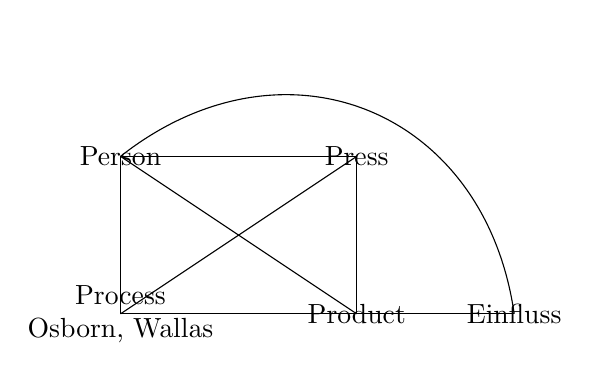
\begin{tikzpicture}
	\begin{pgfonlayer}{nodelayer}
		\node [style=none] (0) at (-8, 3) {Person};
		\node [style=none] (1) at (-5, 3) {Press};
		\node [style=none, align=center] (2) at (-8, 1) {Process \\ Osborn, Wallas};
		\node [style=none] (3) at (-5, 1) {Product};
		\node [style=none] (4) at (-3, 1) {Einfluss};
	\end{pgfonlayer}
	\begin{pgfonlayer}{edgelayer}
		\draw (0.center) to (1.center);
		\draw (0.center) to (2.center);
		\draw (2.center) to (3.center);
		\draw (3.center) to (0.center);
		\draw (2.center) to (1.center);
		\draw (1.center) to (3.center);
		\draw (3.center) to (4.center);
		\draw [bend left=60, looseness=1.25] (0.center) to (4.center);
	\end{pgfonlayer}
\end{tikzpicture}

\begin{tikzcd}
 &  & Person \arrow[dd] \arrow[rr] \arrow[rrdd] &  & Process \arrow[dd] \\
 &  &  &  &  \\
Einfluss \arrow[rr] &  & Produkt \arrow[rr] \arrow[rruu] &  & Press
\end{tikzcd}
\section{Literaturreview}

\begin{mydef}{Literaturreview}{def_lr}
  Im Zuge dieser Arbeit impliziert der Begriff „Wirtschaftsinformatik“ die Betrachtung (konstruierter) IT-Artefakte ausschließlich in Form softwareseitiger Anwendungssysteme.
  This theorem is numbered with  \ref{def:def_lr} and is given on page \pageref{def:def_lr}.
\end{mydef}
\section{Wirtschaftsinformatik}

Der Forschungsbereich der Wirtschaftsinfomratik ist stark durch die beiden paradigmischen Anstäze der Gestaltungs- sowie Verhaltenorientierung geprägt. 
Die Wirtschaftsinformatik sieht sich selbst als interdisziplinare Realwissenschaft, welche Bereiche aus der technischen Perspektive als auch aus der betriebwissenschaftlichen Sichtweise betrachtet und beide verbindet.
Streng genommen weisen die Forschungskulturen der deutschen Wirtschaftsinformatik einerseits und der angloamerikanischen Schwesterdiszplin der Information Systems andererseits große Unterschiede hinsichtlich postulierter Methoden sowie Zielpräferenzen auf. Vor dem Hintergrund der in dieser Arbeit vorrangigen Untersuchung empirischer Evaluationsmethoden ist eine strikte Trennung beider Gebiete in dieser Hinsicht allerdings nicht zwingend notwendig.  Beide Disziplinen unterscheiden zwischen den sich gegenüberstehenden Forschungsparadigmen der Gestaltungsorientierung („Design Science“ im internationalen Raum) und der Erklärungsorientierung („Behaviroul Science“). Die deutsche WI sieht sich dabei stärker auf den praxisorientierteren Gestaltungsansatz fokussiert (Relevanz), wogegen ihr internationale Vertretung den theoretisch geprägten erklärungsorientierten Ansatz in den Vordergrund stellt (Rigor).  Die Ziele der Verhaltensorientierung sind vor allem die des Erklärens und Beschreibens von Zusammenhängen und Theorien (Wahrheitsfindung). Die Hauptfelder gestaltungsorientierter Wirtschaftsinformatik liegen hingegen in der Schaffung und Evaluierung zweckmäßiger Artefakte. Ziel von Design Science ist die Schaffung und Evaluierung zweckbezogener Artefakte zur Lösung von Organisationsproblemen (Simon?) {Frank 1999 #69} Ziel dieser Artefakte ist es, bereits vorhandene Anwendungssysteme zu erweitern oder Probleme zu lösen, die entweder durch informationstechnische Anwendungen zuvor nicht zufriedenstellend gelöst wurden oder konnten. Die Gestaltungsorienteirete Forschung liefert dazu neue Lösungen als IT Artefakt, etwa in Form von Softwareprotytypen, deren Nutzen es im Prozess durch Anwendung geeigneter Forschungsmethoden zu evaluieren gilt. Dabei treten beide Forschungsparadigmen nicht streng dichotom auf, sondern können und müssen sich synergetisch ergänzen. Gerade im Zusammenhang mit dem langen geführten Diskurs zwischen Rigor und Relevanz zeigte sich, dass sich die deutsche Wirtschatfsinformatik zu stark auf den  \label{test}praxisnahen gestaltungsorientioerten Ansatz besinnte. Einerseits wird dieses Vorgehen von vielen Autoren gelobt (Momerndum für die gestatungsorientioere WInfo), andereseits wird auch oft das fehlende theoretische Fundament bemängelt. Gerade im Vergleich zur internationaen Wirtschaftsinformatik, welche sich stärker auf die theorethscihe fundierung bedacht ist, herrsche in der deutschen WI nachholbedarf. Auch die internationale Wi rief mit ihrer klaren Positionierung zur theoretischen Empirie zum Diskurs auf, sprach ihrerseits sogar von einer Identitäskrise (Benbasat und Zmud). Benbast und Zmud kritisierten diesen Fokus und verlangte danach, dass IT-Artefakt in den Mittelpunkt zu stellen und sich auf die Konstruktion nützlicher zu besinnen: Focus should be on how to best design IT artifacts and IS systems to increase their compatibility, usefulness, and ease of use or on how to best manage and support IT or IT-enabled business initiatives.
Das gemeinschaftliche Ziel der deutschen sowie internationalen Wirtschaftsinformatik besteht daher in der Sicherstellung und Steigerung der „Relevanz und Rigor“ Prämisse, also der praxisorientierten gestalterischen Artefaktentwicklung (Gestaltungsorientiert) sowie gleichzeitiger Korrektheit durch Prüfung mittles angemessener theoretischer Fundierung (Erklärungsorientiert). {Alturki 2012 #32: 313} In Anbetracht dieses Ziels gilt es als Aufgabe der Wirtschaftsinfomratik das  richtige Verhältniss im Nutzen beider Forschungsansätze zu finden und implementieren. {Becker 2008 #239: 5}

Der erforderliche Evaluationsschritt innerhalb der DesignScience versucht die Nützlichkeit eines Artefaktes zu „erklären“. Dieser Vorgang ist definitionsgemäß der Behavirolistischen Orientierung zuzuschreiben. Dadurch finden dessen verfügbaren Methoden implizit auch im Gestaltungsprozess Anwendung.  


In der Vergangenheit wurden eine Vielzahl möglicher Klassifikation von IT-Artefakten vorgenommen (Alter?) Die in diesem Zusammenhang jedoch meist genutze war die von HamrchSmith und Hevner dargestellte Unterschidung der Artefakte in: Konstrukte, Modelle, Methode, Instantiierung.
Bei der Definition eines IT-Artefaktes herrscht nach Alter kein kohärentes Verständnis über die genaue Definition eines IT-Atefaktes entwickelt hat, so sprechen sich viele für die von Simon postulierten Definition nach den Arten von Artefakte aus. Diese stellen sich demnachin Form von Konstrukten, Modellen, Methoden oder instatiierungen dar.
Nach Wotawa u. Thierau 1990 kennzeichnet sich die Evaluirung dieser Artefakte durch eine systematische Tätigkeit, welche eine Bewertung einer Sache (Artefakt) nach zweckgerichteter Form vornimmt. Somit dient die Artefaktevaluaiton vornehmlich der Feststellung jender „Nützlichkeit“.

Hess stellte diesen Vorgang schematisch wie in Fig 3 dargestellt auf:




\vspace{1cm}


\begin{mydef}{Wirtschaftsinformatik}{def_wi}
  Im Zuge dieser Arbeit impliziert der Begriff „Wirtschaftsinformatik“ die Betrachtung (konstruierter) IT-Artefakte ausschließlich in Form softwareseitiger Anwendungssysteme.
  This theorem is numbered with  \ref{def:def_wi} and is given on page \pageref{def:def_wi}.
\end{mydef}